\documentclass[aspectratio=1610]{beamer}

\usepackage{fontspec}
\usepackage{tikz}
\usetikzlibrary{arrows.meta,positioning}
\usepackage{booktabs}

\title{Dokazi nultog znanja}
\author{Aleksandra Labović \textbullet{} Matematički fakultet \textbullet{} Univerzitet u Beogradu}
\date{jun 2026}

\usetheme[numbering=progressbar,sectionpage=none]{wildcat}

\setbeamerfont{normal text}{size=\fontsize{18}{22}\selectfont}
\setbeamerfont{frametitle}{size=\fontsize{32}{36}\selectfont}
\setbeamerfont{title}{size=\fontsize{32}{38}\selectfont}
\setbeamerfont{subtitle}{size=\fontsize{18}{22}\selectfont}
\AtBeginEnvironment{frame}{\fontsize{18}{22}\selectfont}

\newcommand{\keyword}[1]{\textcolor{wcprimary}{\textbf{#1}}}
\newcommand{\bigsentence}[1]{{\fontsize{32}{38}\selectfont #1}}
\newcommand{\person}[3]{%
  \begin{scope}[shift={(#1,#2)}]
    \draw[wcprimary, line width=1.4pt] (0,1.35) circle (0.28);
    \draw[wcprimary, line width=1.4pt] (0,1.05) -- (0,0.25);
    \draw[wcprimary, line width=1.4pt] (-0.45,0.75) -- (0.45,0.75);
    \draw[wcprimary, line width=1.4pt] (0,0.25) -- (-0.38,-0.35);
    \draw[wcprimary, line width=1.4pt] (0,0.25) -- (0.38,-0.35);
    \node[font=\large] at (0,-0.85) {#3};
  \end{scope}%
}

\begin{document}

\begin{frame}
  \titlepage
\end{frame}

\begin{frame}{Zašto uopšte postoji problem?}
\begin{block}{Situacija}
  Alisa ima lozinku, Bob administrira server.
\end{block}
\vspace{6pt}
\begin{alertblock}{Problem}
  Kako dokazati da posedujemo određenu informaciju, a da pritom ne otkrijemo njen sadržaj?
\end{alertblock}
\vspace{6pt}
\begin{exampleblock}{Naivno rešenje}
  Delimično otkrivanje pojedinih karaktera lozinke ne rešava problem.\\
  Verifikator i dalje postepeno uči delove tajne.
\end{exampleblock}
\end{frame}

\begin{frame}{Šta su dokazi nultog znanja?}
\begin{columns}
  \begin{column}{0.5\textwidth}
    \begin{itemize}
      \setlength{\itemsep}{12pt}
      \item Goldwasser, Micali, Rackoff \\ MIT i Univerzitet Toronto, 1985.
      \item \textit{The Knowledge Complexity of Interactive Proof-Systems}
      \item Konferencija \keyword{STOC}, jedna od najznačajnijih konferencija iz oblasti teorijskog računarstva
    \end{itemize}
  \end{column}
  \begin{column}{0.45\textwidth}
    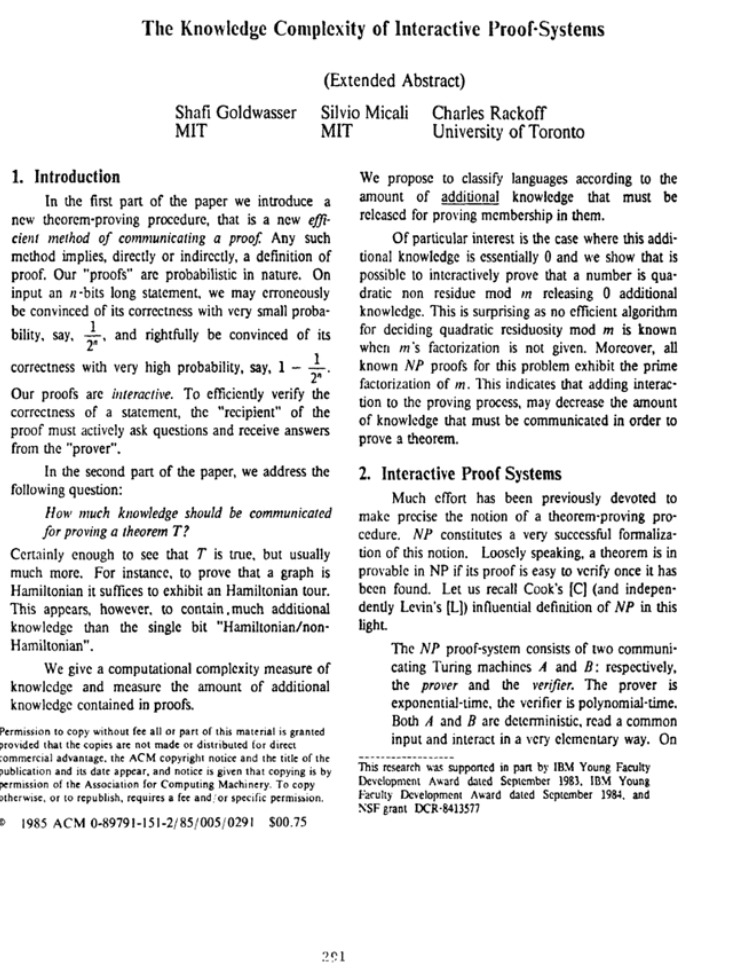
\includegraphics[width=\textwidth]{zkp_rad.jpeg}
  \end{column}
\end{columns}
\end{frame}

\begin{frame}{Dokazivač i verifikator}
\begin{center}
\large
\begin{tabular}{p{0.47\textwidth} p{0.42\textwidth}}
  \begin{block}{Dokazivač (Peggy)}
    Strana koja tvrdi da poseduje određenu informaciju i želi da u to uveri verifikatora.
  \end{block}
  &
  \begin{block}{Verifikator (Viktor)}
    Strana koja proverava da li je tvrdnja tačna.
  \end{block}
\end{tabular}
\end{center}
\vspace{12pt}
\begin{alertblock}{\centering Idealni cilj}
  \centering
  Verifikator se uverava u tačnost tvrdnje, ali \keyword{ne saznaje ništa o samoj tajni}.
\end{alertblock}
\end{frame}

\begin{frame}{Primer: Izomorfizam grafova}
\begin{center}
  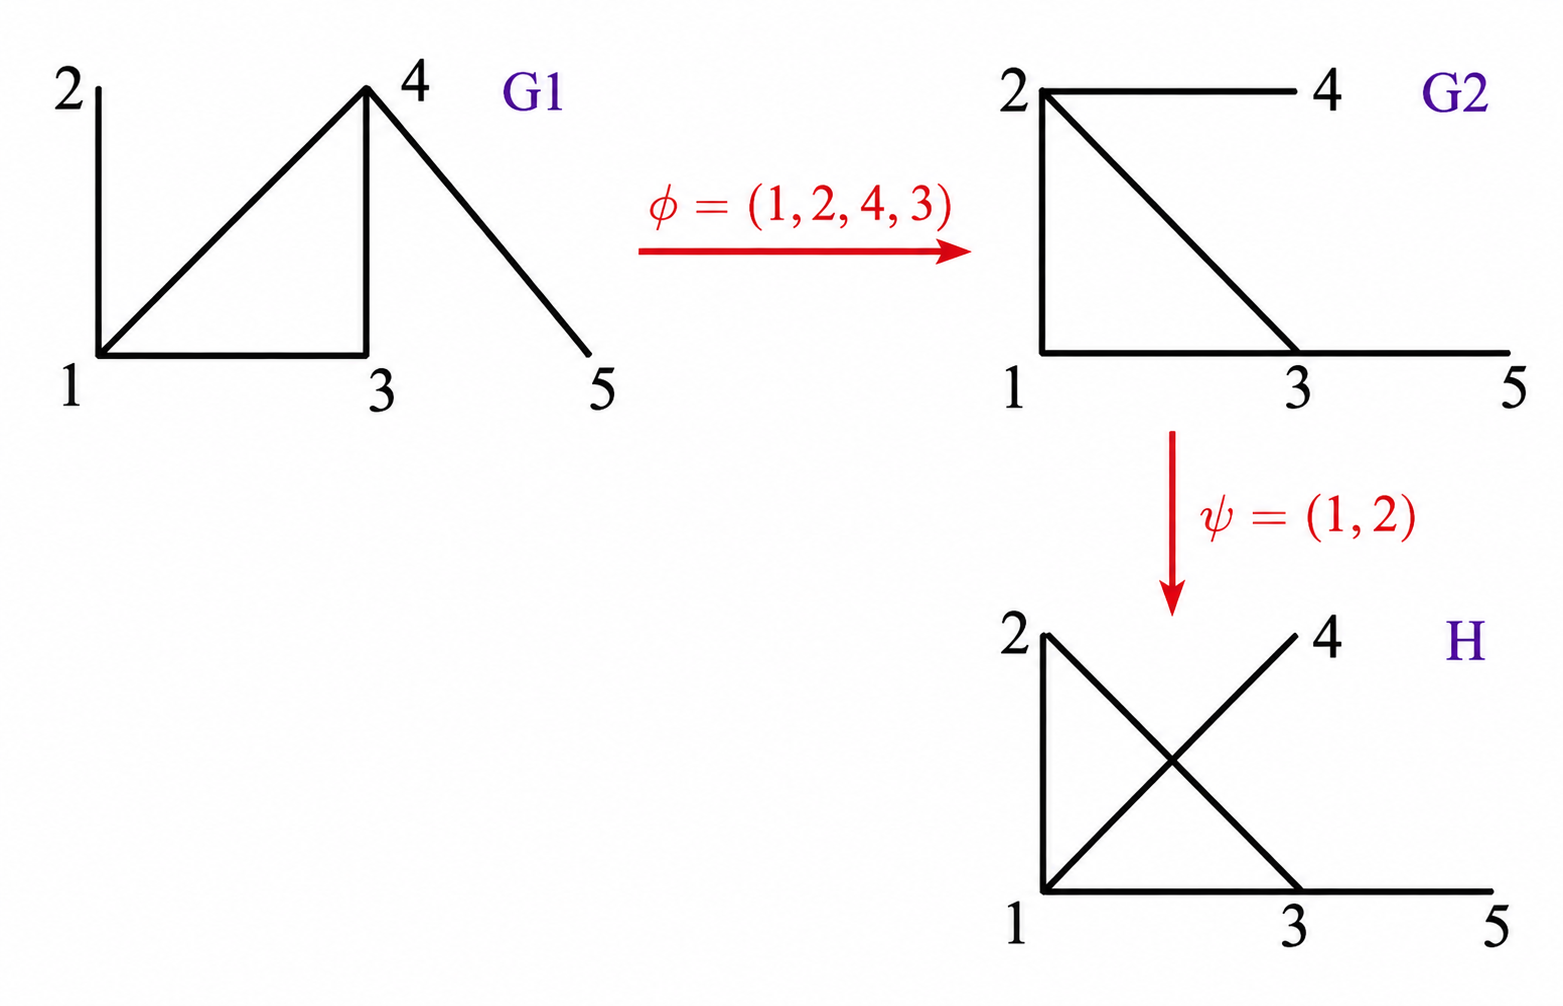
\includegraphics[width=0.85\textwidth]{graf_izomorfizam.png}
\end{center}
\vspace{-8pt}
\begin{columns}
  \begin{column}{0.5\textwidth}
    \begin{itemize}
      \item $G_1$ i $G_2$ su \keyword{izomorfni}
    \end{itemize}
  \end{column}
  \begin{column}{0.5\textwidth}
    \begin{itemize}
      \item Pegi poznaje izomorfizam $\varphi = (1,2,4,3)$, dok ga Viktor ne poznaje
    \end{itemize}
  \end{column}
\end{columns}
\end{frame}

\begin{frame}{Tok protokola}
\begin{enumerate}
  \setlength{\itemsep}{10pt}
  \item \keyword{Posveta.} Pegi bira slučajnu permutaciju $\psi$ i konstruiše
  \[ H \leftarrow \psi(G_2) \]
  Dobijeni graf $H$ šalje Viktoru.

  \item \keyword{Izazov.} Viktor bira $b \in \{1, 2\}$ nasumično i traži
  izomorfizam između $G_b$ i $H$.

  \item \keyword{Odgovor.} Pegi šalje
  \[
    \chi = \begin{cases} \psi & \text{ako } b = 2 \\ \psi \circ \varphi & \text{ako } b = 1 \end{cases}
  \]

  \item \keyword{Provera.} Viktor prihvata ako važi $\chi(G_b) = H$.
\end{enumerate}
\end{frame}

\begin{frame}{Zašto protokol radi?}
\vspace{-4pt}

\begin{block}{Potpunost}
  Pegi poznaje $\varphi$, pa za svaki Viktorov izazov može poslati
  odgovarajući izomorfizam.
\end{block}

\vspace{-3pt}

\begin{alertblock}{Tačnost}
  Lažna Pegi mora unapred pogoditi Viktorov izazov.
  Verovatnoća uspeha nakon $20$ rundi iznosi manje od
  $0{,}000001$, odnosno manja je od jedne u milion.
\end{alertblock}

\vspace{-3pt}

\begin{exampleblock}{Važno}
  Ako bi se isti $H$ koristio dva puta, Viktor bi mogao iz odgovora
  $\psi$ i $\psi \circ \varphi$ izračunati
  $\varphi = (\psi \circ \varphi)\circ\psi^{-1}$.
\end{exampleblock}

\end{frame}

\begin{frame}{Tri ključna svojstva}
\vspace{4pt}
\begin{block}{\normalsize Potpunost \textnormal{(engl.\ \textit{completeness})}}
  Ako dokazivač poseduje traženo znanje i pošteno prati protokol, verifikator prihvata dokaz.
\end{block}
\begin{alertblock}{\normalsize Tačnost \textnormal{(engl.\ \textit{soundness})}}
  Dokazivač koji ne poseduje traženo znanje može uspeti samo sa zanemarljivo malom verovatnoćom.
\end{alertblock}
\begin{exampleblock}{\normalsize Nulto znanje \textnormal{(engl.\ \textit{zero-knowledge})}}
  Viktor može sam da generiše transkript koji izgleda kao stvarna
  komunikacija sa Pegi, bez poznavanja izomorfizma $\varphi$.
  Pošto se takav transkript ne može razlikovati od stvarnog,
  protokol ne otkriva nikakvu informaciju o $\varphi$.
\end{exampleblock}
\end{frame}

\begin{frame}{Tri nivoa nultog znanja}
\vspace{4pt}
Neka je $V$ skup stvarnih transkripata, a $S$ skup simuliranih.
\begin{block}{\normalsize Savršeno nulto znanje \textnormal{($V = S$)}}
  Raspodele su \keyword{identične} pa ni neograničen protivnik ne može razlikovati\\
  simulirani transkript od stvarnog. Primer: izomorfizam grafova.
\end{block}
\begin{alertblock}{\normalsize Statističko nulto znanje \textnormal{($V \approx_s S$)}}
  Raspodele se razlikuju za statistički zanemarljivu vrednost, odsnono\\
  neraspoznatljive su čak i za neograničenog protivnika.
\end{alertblock}
\begin{exampleblock}{\normalsize Računsko nulto znanje \textnormal{($V \approx_c S$)}}
  Raspodele su za \keyword{računski ograničenog} protivnika statistički neodvojive.
  U ovu kategoriju spada većina praktičnih protokola.
\end{exampleblock}
\end{frame}

\begin{frame}{Veza sa teorijom složenosti}
\vspace{4pt}
\begin{block}{\normalsize $\mathbf{NP}$}
  Postoji kratak \keyword{svedok} čiju ispravnost računski ograničen verifikator
  može proveriti u polinomskom vremenu, bez interakcije sa dokazivačem.
\end{block}
\begin{alertblock}{\normalsize $\mathbf{IP}$}
  Neograničen dokazivač i ograničen verifikator razmenjuju poruke u više rundi.
  \[
    \mathbf{IP} = \mathbf{PSPACE}
  \]
\end{alertblock}
\begin{exampleblock}{\normalsize $\mathbf{CZK}$}
  Skup problema dokazivih uz računsko nulto znanje.
  Već smo pokazali da izomorfizam grafova leži u $\mathbf{CZK}$.
  Koliko je ova klasa velika?
\end{exampleblock}
\end{frame}

\begin{frame}{$\mathbf{NP} \subseteq \mathbf{CZK}$}
\begin{block}{\normalsize 3-obojivost}
  Može li se svaki čvor obojiti jednom od tri boje tako da nijedna grana
  ne spaja čvorove \keyword{iste boje}? Ovaj problem je NP-kompletan.
\end{block}
\begin{alertblock}{\normalsize Protokol}
  \begin{enumerate}\itemsep2pt
    \item Pegi objavljuje posvete na permutovane boje čvorova
    \item Viktor bira jednu granu
    \item Pegi otkriva boje njenih krajeva pa Viktor proverava da li su različite
  \end{enumerate}
\end{alertblock}
\begin{exampleblock}{\normalsize Posledica}
  Pošto je 3-obojivost NP-kompletna, sledi $\mathbf{NP} \subseteq \mathbf{CZK}$.
  Svaka NP tvrdnja je dokaziva uz nulto znanje.
\end{exampleblock}
\end{frame}

\begin{frame}{Sigma protokoli}
\vspace{6pt}
\begin{center}
\large
$\underbrace{\text{posveta}}_{P \to V}
\quad \longrightarrow \quad
\underbrace{\text{izazov}}_{V \to P}
\quad \longrightarrow \quad
\underbrace{\text{odgovor}}_{P \to V}$
\end{center}
\vspace{8pt}
\begin{block}{\normalsize Karakteristike}
  \begin{itemize}\itemsep6pt
    \item Klasa efikasnih ZK protokola zasnovanih na algebarskim problemima.
    \item Pretpostavka \keyword{poštenog verifikatora} pojednostavljuje analizu
  \end{itemize}
\end{block}
\vspace{6pt}
\begin{exampleblock}{\normalsize Najpoznatiji primer}
  \textbf{Schnorr-ov identifikacioni protokol} zasnovan na problemu\\ diskretnog logaritma
\end{exampleblock}
\end{frame}

\begin{frame}{Schnorr-ov protokol}
\vspace{6pt}
Grupa $G$ prostog reda $q$, generator $g$, javna vrednost $y = g^x$. Pegi zna $x$.
\vspace{10pt}
\[
  \begin{array}{rcl}
    P \to V & : & r \leftarrow g^k, \quad k \xleftarrow{R} \mathbb{Z}_q \\[10pt]
    V \to P & : & e \xleftarrow{R} \mathbb{Z}_q \\[10pt]
    P \to V & : & s \leftarrow k + x \cdot e \pmod{q}
  \end{array}
\]
\vspace{6pt}
\begin{block}{\normalsize Provera}
  \[
    g^s \cdot y^{-e} = g^{k+xe} \cdot g^{-xe} = g^k = r \quad \checkmark
  \]
\end{block}
\vspace{6pt}
{\small Verovatnoća prevare iznosi $\dfrac{1}{q}$, što obezbeđuje \keyword{jaku bezbednost} već u jednoj rundi.}
\end{frame}

\begin{frame}{Chaum-Pedersen protokol}
\vspace{4pt}
Cilj je dokazati da postoji $x$ takvo da $y_1 = g^x$ i $y_2 = h^x$,
tj.\ da važi $\log_g y_1 = \log_h y_2$.
\vspace{8pt}
\[
  \begin{array}{rcl}
    P \to V & : & (r_1, r_2) \leftarrow (g^k,\, h^k), \quad k \xleftarrow{R} \mathbb{Z}_q \\[10pt]
    V \to P & : & e \xleftarrow{R} \mathbb{Z}_q \\[10pt]
    P \to V & : & s \leftarrow k - e \cdot x \pmod{q}
  \end{array}
\]
\vspace{6pt}
\begin{block}{\normalsize Provera}
  \[
    r_1 = g^s \cdot y_1^e \qquad \text{i} \qquad r_2 = h^s \cdot y_2^e
  \]
\end{block}
\vspace{6pt}
{\small Prvobitno razvijen za \keyword{elektronski novac}, danas predstavlja važan gradivni element brojnih kriptografskih protokola.}
\end{frame}

\begin{frame}{Fiat-Shamir heuristika}
\vspace{4pt}
{\small Pegi želi da objavi dokaz koji će svako moći da proveri, bez direktne komunikacije sa verifikatorom.}
\begin{block}{\normalsize Ideja}
  Verifikatorov nasumični izazov zamenjujemo \keyword{heš-vrednošću} javnih podataka:
  \[
    e = H(r \,\|\, g \,\|\, y)
  \]
  Uključivanje $g$ i $y$ vezuje dokaz za konkretnu tvrdnju i konkretne parametre.
\end{block}
\begin{exampleblock}{\normalsize Primena: digitalni potpisi}
  Potpis poruke $m$ predstavlja ZK dokaz znanja tajnog ključa:
  \[
    e = H(r \,\|\, g \,\|\, y \,\|\, m)
  \]
\end{exampleblock}
\end{frame}

\begin{frame}{Elektronsko glasanje}
\vspace{4pt}
{\small $m$ glasača, $n$ centara za prebrojavanje. Rezultat je \keyword{javno proverljiv}, glasovi su \keyword{trajno skriveni}.}
\vspace{8pt}
\begin{enumerate}\itemsep8pt
  \item \keyword{Posveta glasa.}
  Glasač objavljuje Pedersen-ovu posvetu koja skriva vrednost glasa.

  \item \keyword{ZK dokaz validnosti.}
  Neinteraktivni dokaz da je glas jedna od dve dozvoljene opcije,
  bez otkrivanja koja.

  \item \keyword{Tajno deljenje.}
  Glasač deli tajnu između $n$ centara po Shamir-ovoj šemi.
  Nijedan centar ne može sam rekonstruisati glas.

  \item \keyword{Prebrojavanje.}
  Svaki centar objavljuje sumu svojih udela.
  Rezultat se dobija interpolacijom.
\end{enumerate}
\end{frame}

\begin{frame}{Zaključak}
\vspace{10pt}
\begin{itemize}\itemsep10pt
  \item ZKP omogućavaju dokazivanje istinitosti \keyword{bez otkrivanja} ikakve informacije
  \item Svaka NP tvrdnja je dokaziva uz nulto znanje: $\mathbf{NP} \subseteq \mathbf{CZK}$
  \item Uz pretpostavku jednosmernih funkcija važi $\mathbf{CZK} = \mathbf{IP} = \mathbf{PSPACE}$
  \item Primene obuhvataju autentifikaciju, digitalne potpise, elektronsko glasanje i savremene blokčejn sisteme
\end{itemize}
\end{frame}

\begin{frame}{}
\begin{center}
  \Huge Hvala na pažnji!
\end{center}
\end{frame}

\end{document}